Visualization (0.5 page) (AJ, JP)
\begin{itemize}
  \item Transparency
	\item Opacity mapping (surface, AO, ...)
\end{itemize}

Interactive Analysis (0.5 page) (ALL)
\begin{itemize}
  \item Possibilities (scenario, dynamics, pipeline)
  \item Feedback
\end{itemize}

\subsection{Rendering of spherical patches --- polygons?}
\label{sec:spherical-patches}
A sphere can produce one or more spherical patches which may form different surfaces.
To be able to visualize isolated surfaces individually, we render (ray-cast) each spherical patch as a separate surface primitive.
This way, we are able to visually distinguish between molecular and cavity surface and also among the detected cavities themselves.
In fact, the sides of a spherical patch are formed by small circle arcs.
When ray-casting a spherical patch, we firstly compute intersection points $I_1$ and $I_2$ of a ray and patch's sphere.
Then, we employ the odd-even rule to test whether the computed intersections lie within the patch.
We choose a point $O$ outside the patch and test lines (lying on a great circle) $OI_1$ and $OI_2$ for intersection with each side of the patch.
The outside (or inside) point must be specified because both the interior and exterior surfaces of the sphere are finite.

\begin{figure}[htb]
  \centering
  \includegraphics[width=1.5in]{image/patch.png}
  \caption{Point spherical patch test.}
\end{figure}

The intersection of a spherical segment with a small circle arc is computed in three steps:
\begin{enumerate}
  \item The intersection of the circles containing the segment and the arc is computed --- they can intersect in 0 to 2 points.
  \item The intersection points are tested whether they lie on both the segment and the arc.
  \item Cases with two intersections are marked as non-intersecting because the tested point lies outside the patch.
\end{enumerate}

\textcolor{red}{TODO: \textsc{http://horizon.documentation.ird.fr/exl-doc/pleins\_textes/pleins\_textes\_6/b\_fdi\_39-40/43404.pdf}}

\subsection{Cavity area estimation}
Observation: triangles take most area of a cavity.

We enhance the visualization of cavities by coloring their surface by their approximate area.
To estimate the area, we sum areas of all triangles that form the cavity surface.
Therefore, the cavity area we compute is \textcolor{red}{underestimated -- maybe an equation?}.
We decided to neglect areas of spherical and toroidal patches since from our observations their influence on the exact cavity area is much smaller compared to triangles.
Of course, this observation does not hold for the molecular surface.
\textcolor{red}{What about coloring?}
